\documentclass[11pt,a4paper]{article}

% --- Packages ---
\usepackage[utf8]{inputenc}
\usepackage[english]{babel}
\usepackage{amsmath, amssymb, amsfonts, bm}
\usepackage{geometry}
\usepackage{graphicx}
\usepackage{subcaption}
\usepackage{booktabs}
\usepackage{hyperref}
\usepackage{cite}
\usepackage{float}
\usepackage{xcolor}
\usepackage{enumitem}
\usepackage{tikz}
\usetikzlibrary{arrows.meta, positioning, calc, fit}

\geometry{a4paper, top=2.5cm, bottom=2.5cm, left=2.5cm, right=2.5cm}
\setlength{\emergencystretch}{3em}

\hypersetup{
    colorlinks=true,
    linkcolor=blue!70!black,
    citecolor=green!50!black,
    urlcolor=cyan!70!black
}

% --- Macros ---
\newcommand{\bq}{\bm{q}}
\newcommand{\bdq}{\dot{\bm{q}}}
\newcommand{\bddq}{\ddot{\bm{q}}}
\newcommand{\btau}{\bm{\tau}}
\newcommand{\bM}{\bm{M}}
\newcommand{\bC}{\bm{C}}
\newcommand{\bG}{\bm{G}}
\newcommand{\bB}{\bm{B}}
\newcommand{\Real}{\mathbb{R}}
\newcommand{\dgr}{^{\circ}}

% --- Colours and diagram styles (same palette as the slides) ---
\definecolor{pidred}{HTML}{C0392B}
\definecolor{mpcteal}{HTML}{1F6F78}
\definecolor{slate}{HTML}{4A6274}
\definecolor{ink}{HTML}{263238}
\tikzset{
    blk/.style={draw=slate, fill=slate!8, rounded corners=2pt, align=center, font=\footnotesize,
                minimum height=1.0cm, inner sep=3pt},
    pidblk/.style={blk, draw=pidred, fill=pidred!12},
    mpcblk/.style={blk, draw=mpcteal, fill=mpcteal!12},
    outblk/.style={blk, draw=ink, fill=ink, text=white, font=\footnotesize\bfseries},
    arr/.style={-{Latex[length=2mm]}, thick, slate},
    todo/.style={draw=slate, dashed, rounded corners=3pt, fill=slate!5, align=center,
                 text width=0.42\linewidth, minimum height=4.2cm, font=\footnotesize}
}

% ============================================================
\begin{document}

\begin{titlepage}
    \centering
    \vspace*{2cm}
    {\Large\bfseries Field and Service Robotics --- Final Technical Report\par}
    \vspace{1.5cm}
    {\LARGE\bfseries Modeling and Control of the RoTino Wheeled Biped:\\[6pt]
    ZMP-Based PID and MPC + TV-LQR\par}
    \vspace{1cm}
    {\large Euler--Lagrange Dynamics, Configuration Space,\\ Controller Design and Comparison Framework\par}
    \vspace{2cm}
    {\large Aldo Rosicarelli \quad Alessando Prisco\par}
    \vspace{0.5cm}
    {\large Academic Year 2025--2026\par}
    \vfill
    {\large Field and Service Robotics\par}
\end{titlepage}

% ============================================================
\tableofcontents
\newpage

% ============================================================
\section{Introduction}
\label{sec:intro}

Wheeled biped robots combine the mobility and energy efficiency of wheeled platforms with the
postural versatility of legged systems.  By changing the length of their legs they move the
height at which the upper-body mass is carried, which makes them a \emph{Variable-Length
Wheeled Inverted Pendulum} (VL-WIP).  The control problem is hard for two structural reasons:
the system is \emph{underactuated}, since the pitch of the upper body has no actuator of its
own and must be steered through the wheels, and it is \emph{non-minimum phase}, since to
accelerate forward the wheels must first move backwards under a forward-leaning body.

The platform studied here is \textbf{RoTino}, a 4.29~kg wheeled biped simulated in Gazebo
Fortress with ROS~2 Humble and torque-controlled through \texttt{ros2\_control} at 500~Hz.
Two control laws are designed and compared on the same robot, world and actuation:

\begin{enumerate}[leftmargin=*]
    \item a \textbf{cascade PID built around the Zero Moment Point} (ZMP), in which the wheels
          place the ZMP and a capture-point loop decides where it should be
          (package \texttt{rotino\_pid});
    \item the \textbf{MPC + TV-LQR + VMC} architecture of Cui et al.~\cite{cui2022}, in which a
          gain-scheduled LQR balances the pendulum, a constrained MPC plans the upper-body motion
          and a virtual model controller drives the legs (package \texttt{rotino\_mpc}).
\end{enumerate}

With respect to the previous version of this report, the sliding mode controller has been
removed from the project, the PID has been redesigned around the ZMP, and the dynamic model is
derived with the parameters of the RoTino URDF instead of those of the robot of the paper.
The symbolic model follows the structure of the MATLAB script \texttt{Matlab/SMC/init.m} and
is recomputed in SymPy (\texttt{docs/presentazione/modello\_lagrangiano.py}), which also checks
its properties automatically.

The report is structured as follows.  Section~\ref{sec:params} lists the modelling
assumptions and parameters.  Section~\ref{sec:topology} analyses the degrees of freedom and
the topology of the configuration space.  Section~\ref{sec:model} derives the dynamic model.
Sections~\ref{sec:pid} and~\ref{sec:lqr_mpc} describe the two controllers.
Section~\ref{sec:comparison} sets up the comparison framework.  Section~\ref{sec:conclusions}
concludes.


% ============================================================
\section{Robot Parameters and Modelling Assumptions}
\label{sec:params}

\subsection{Physical Parameters}

All parameters are read from the URDF (\texttt{rotino\_description/urdf/rotino.urdf.xacro})
by the \texttt{WBRModel} class: no value is copied by hand into the controllers.

\begin{table}[H]
    \centering
    \caption{Physical parameters of RoTino (per side unless stated otherwise).}
    \label{tab:params}
    \begin{tabular}{llp{6.3cm}}
        \toprule
        Symbol & Value & Origin \\
        \midrule
        $m_w$ & 0.38~kg & wheel 0.32 + hub 0.06 \\
        $I_w$ & $2.595\cdot10^{-3}$~kg\,m$^2$ & wheel $i_{yy}$, including the MuJoCo armature \\
        $r$, $d$ & 0.06~m, 0.294~m & wheel radius, track \\
        $m_b$ & 3.53~kg & total mass (4.29~kg) minus the two wheels \\
        $m_3$ & 2.85~kg & torso 2.50 + ballast 0.35 \\
        $m_2$, $m_1$ & 0.18~kg, 0.16~kg & thigh, shank \\
        $l_1 = l_2$ & 0.130~m & $\sqrt{2}\cdot 0.0919$: segments inclined at $45\dgr$ \\
        $\mu$ & 2.2 & wheel--ground friction \\
        $\tau_{w,max}$, $\tau_{leg,max}$ & 18~Nm, 60~Nm & URDF limits (both controllers use 10~Nm on the wheels) \\
        \bottomrule
    \end{tabular}
\end{table}

Three features of the robot weigh on the control design:
\begin{enumerate}[leftmargin=*]
    \item \textbf{Heavy rolling wheels.}  $2I_w/r^2 = 1.44$~kg: the rotational inertia of the
          wheels, reflected to translation, is 41\% of $m_b$ and cannot be neglected.
    \item \textbf{Forward torso CoM.}  The torso CoM lies at $(+27.5;\,-5.5)$~mm from the hip;
          at equilibrium the torso must therefore be tilted backwards by about $4.7\dgr$.
    \item \textbf{Smaller real inertia.}  The inertia of the upper body about its CoM, computed
          from the URDF tensors, is $I_y = 0.0174$~kg\,m$^2$, whereas Table~1 of~\cite{cui2022}
          assumes $m_b l^2/3 = 0.0311$~kg\,m$^2$ (1.8 times larger).
\end{enumerate}

\subsection{Modelling Assumptions}

\begin{itemize}[leftmargin=*]
    \item \textbf{Sagittal plane.}  The two legs move together and are lumped: leg and wheel
          masses and inertias count twice, the torso once.
    \item \textbf{Rigid bodies, ideal joints.}  Shank and thigh are rods with the CoM at
          mid-length; the torso CoM is at $(a_3, b_3)$ in the torso frame.
    \item \textbf{Pure rolling on flat ground.}  $s_w = r\,q_w$, no slip, no lift-off.
    \item \textbf{Torque actuation.}  Wheels, knees and hips receive direct torques
          (\texttt{effort} command interface).
\end{itemize}
Neglected effects: yaw and roll (treated separately), wheel slip and contact loss, joint
damping (0.8~Nm\,s/rad, compensated in feedforward by both controllers), motor dynamics and
sampling, camber and width of the cylindrical wheel (56~mm).


% ============================================================
\section{Topology Analysis and Degrees of Freedom}
\label{sec:topology}

\subsection{DOF Count}

Before imposing the ground contact, the robot is a floating base with six joints:
\begin{equation}
    n = \underbrace{6}_{\text{torso}} + \underbrace{2}_{\text{hips}} + \underbrace{2}_{\text{knees}}
      + \underbrace{2}_{\text{wheels}} = 12,
    \qquad
    \bq = [x, y, z, \phi, \theta, \psi,\ q_{hl}, q_{hr},\ q_{kl}, q_{kr},\ q_{wl}, q_{wr}]^T .
\end{equation}
The torso is a free rigid body (three translations and three rotations); hips and knees are
revolute joints limited to $\pm0.9$~rad; the wheels are continuous joints.

\subsection{Topology of the Configuration Space}

Spaces with the same number of DOFs are not necessarily equivalent topologically.  For RoTino
\begin{equation}
    \mathcal{C} = SE(3)\times\Real^4\times T^2
    \;\cong\; \Real^3\times SO(3)\times[q^-,q^+]^4\times S^1\times S^1 .
\end{equation}
The torso lives in $SE(3)$, and $SO(3)$ is represented with quaternions to avoid the gimbal
lock.  Hips and knees have mechanical limits: each joint is a closed interval, not a circle,
hence $\Real^4$.  The wheels rotate without limits: two circles, i.e.\ a torus $T^2$.
$\Real^{12}$ and $\mathcal{C}$ cannot be deformed into each other.

\subsection{Holonomic and Non-Holonomic Constraints}

When the wheels touch the ground two kinds of constraints appear.  The \emph{holonomic} ones
(flat ground: axle height fixed at $r$, roll tied to the legs) reduce the number of
coordinates.  The \emph{non-holonomic} ones, in Pfaffian form $A^T(\bq)\bdq = 0$, express
rolling without slipping:
\begin{align}
    \dot x\sin\psi - \dot y\cos\psi &= 0 \quad\text{(no lateral slip)},\\
    \dot x\cos\psi + \dot y\sin\psi = \tfrac{r}{2}(\omega_l+\omega_r), &\qquad
    \dot\psi = \tfrac{r}{d}(\omega_r-\omega_l).
\end{align}
They restrict the admissible velocities but not the reachable configurations, since the Lie
brackets of the input vector fields span the tangent space.  The constraint reactions enter
the dynamics through Lagrange multipliers:
\begin{equation}
    \bM(\bq)\bddq + \bm{h}(\bq,\bdq) = \bB(\bq)\btau + A(\bq)\bm{\lambda}.
\end{equation}

\textbf{Brockett's theorem~\cite{brockett1983}.}  The differential-drive (unicycle) model admits no smooth,
time-invariant feedback that asymptotically stabilises a point $(x_d, y_d, \psi_d)$.  Both
controllers therefore stabilise the balance and \emph{track trajectories in time} rather than
parking on a pose.

\subsection{Underactuation at Three Levels}

Underactuation is a property of the model in use.  Table~\ref{tab:underact} lists the three
models that appear in this report.

\begin{table}[H]
    \centering
    \caption{Coordinates and actuators of the three models.}
    \label{tab:underact}
    \begin{tabular}{lccp{7cm}}
        \toprule
        Model & $n$ & $m$ & Remark \\
        \midrule
        Free robot & 12 & 6 & wheels, knees, hips; $\operatorname{rank}\bB = 6 < n$ \\
        Planar model (Sec.~\ref{sec:model}) & 4 & 3 & $q_1$ has no motor; the motor reactions move it (non-collocated) \\
        Sagittal VL-WIP & 2 & 1 & $s$ and $\theta$ with the single input $u=\tau_l+\tau_r$ \\
        \bottomrule
    \end{tabular}
\end{table}

The consequence for control is that \emph{to move forward the robot must first lean}: the
lean angle, or equivalently the ZMP, is the virtual input of the translation.  The two
controllers differ in how they choose it: the PID through the ZMP, the MPC through the CoM
offset $\Delta s$.


% ============================================================
\section{Dynamic Model}
\label{sec:model}

\subsection{Generalised Coordinates}

The planar model uses the four coordinates of \texttt{init.m} (Fig.~\ref{fig:coords}):
\begin{equation}
    \bq = [q_1,\ q_w,\ q_2,\ q_3]^T
\end{equation}
where $q_1$ is the absolute shank angle from the horizontal (passive), $q_w$ the absolute
wheel rotation ($s_w = r q_w$, actuated by $\tau_w$), $q_2$ the relative knee angle
(thigh $= q_1+q_2$, actuated by $\tau_k$) and $q_3$ the absolute torso pitch from the vertical
(actuated by the hip torque $\tau_h$).  In the nominal pose of RoTino (all URDF joints at zero)
$q_1 = 135\dgr$, $q_2 = -90\dgr$, $q_3 = 0$: the shank rises backwards and the thigh comes
forward, so that the wheel lies exactly under the hip.  The mapping from the URDF joints is
$q_1 = 135\dgr - (\theta_{pitch} + q_{hip} + q_{knee})$, $q_2 = q_{knee} - 90\dgr$,
$q_3 = \theta_{pitch}$.

\begin{figure}[H]
    \centering
    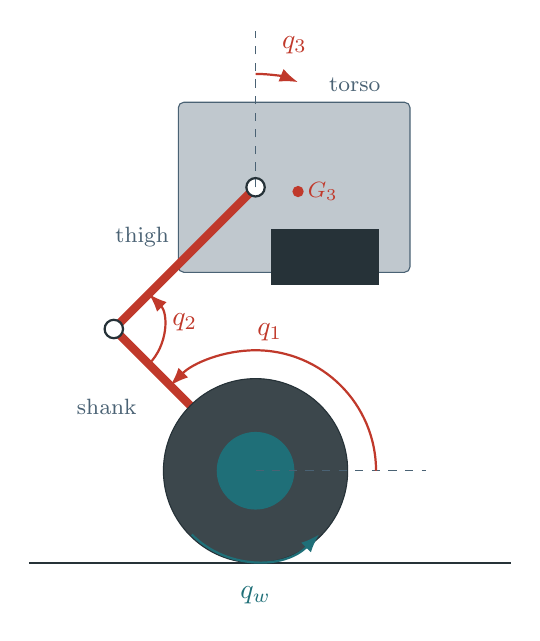
\begin{tikzpicture}[scale=0.9]
        \draw[thick, ink] (-3.2,-1.3) -- (3.6,-1.3);
        % torso and ballast
        \draw[fill=slate!35, draw=slate, rounded corners=2pt] (-1.09,2.8) rectangle (2.18,5.2);
        \draw[fill=ink, draw=ink] (0.22,2.63) rectangle (1.74,3.41);
        % legs
        \draw[line width=3pt, pidred] (0,0) -- (-2,2) -- (0,4);
        % wheel
        \draw[fill=ink!90, draw=ink] (0,0) circle (1.3);
        \draw[fill=mpcteal, draw=mpcteal] (0,0) circle (0.54);
        \foreach \p in {(-2,2),(0,4)} \draw[fill=white, draw=ink, thick] \p circle (0.13);
        % references and angles
        \draw[dashed, slate] (0,0) -- (2.4,0);
        \draw[dashed, slate] (0,4) -- (0,6.2);
        \draw[pidred, thick, -{Latex}] (1.7,0) arc (0:135:1.7);
        \node[pidred] at (0.2,1.95) {$q_1$};
        \draw[pidred, thick, -{Latex}] ($(-2,2)+(-45:0.7)$) arc (-45:45:0.7);
        \node[pidred] at (-1.0,2.1) {$q_2$};
        \draw[pidred, thick, -{Latex}] (0,5.6) arc (90:68:1.6);
        \node[pidred] at (0.55,6.0) {$q_3$};
        \draw[mpcteal, thick, -{Latex}] (-0.9,-0.9) arc (225:315:1.27);
        \node[mpcteal] at (0,-1.75) {$q_w$};
        \node[slate, font=\footnotesize] at (-2.1,0.9) {shank};
        \node[slate, font=\footnotesize] at (-1.6,3.3) {thigh};
        \node[slate, font=\footnotesize] at (1.4,5.45) {torso};
        \fill[pidred] (0.6,3.94) circle (0.08) node[right, font=\footnotesize] {$G_3$};
    \end{tikzpicture}
    \caption{Planar model of RoTino in the nominal pose (to scale): generalised coordinates and
    torso CoM $G_3$.  $q_1$ and $q_2$ are counter-clockwise, $q_3$ and $q_w$ clockwise
    (forward), as in \texttt{init.m}.}
    \label{fig:coords}
\end{figure}

\subsection{CoM Kinematics and Energies}

Starting from the wheel centre, the CoM positions are written along the chain:
\begin{align}
    \bm{p}_1 &= \begin{bmatrix} s_w\\0\end{bmatrix} + \tfrac{l_1}{2}\begin{bmatrix}\cos q_1\\ \sin q_1\end{bmatrix}, &
    \bm{p}_k &= \begin{bmatrix} s_w\\0\end{bmatrix} + l_1\begin{bmatrix}\cos q_1\\ \sin q_1\end{bmatrix},\\
    \bm{p}_2 &= \bm{p}_k + \tfrac{l_2}{2}\begin{bmatrix}\cos q_{12}\\ \sin q_{12}\end{bmatrix}, &
    \bm{p}_h &= \bm{p}_k + l_2\begin{bmatrix}\cos q_{12}\\ \sin q_{12}\end{bmatrix},\\
    \bm{p}_3 &= \bm{p}_h + a_3\begin{bmatrix}\cos q_3\\ -\sin q_3\end{bmatrix} + b_3\begin{bmatrix}\sin q_3\\ \cos q_3\end{bmatrix}, &
    q_{12} &= q_1 + q_2 .
\end{align}
The only difference with \texttt{init.m} is the last line: the torso CoM is shifted by
$(a_3, b_3) = (+27.5;\,-5.5)$~mm in the torso frame instead of lying at $l_3/2$ above the hip.
The kinetic and potential energies are
\begin{align}
    T &= \tfrac12\big(m_w r^2 + I_w\big)\dot q_w^2 + \sum_{i=1}^{3}\tfrac12 m_i\,\dot{\bm p}_i^T\dot{\bm p}_i\nonumber\\
      &\quad + \tfrac12 I_1\dot q_1^2 + \tfrac12 I_2(\dot q_1+\dot q_2)^2 + \tfrac12 I_3\dot q_3^2,\\
    U &= m_w g r + \sum_{i=1}^{3} m_i\,g\,(r + y_i), \qquad \mathcal{L} = T - U,
\end{align}
with $\dot{\bm p}_i = (\partial\bm p_i/\partial\bq)\,\bdq$.  With the legs lumped, the parameters
are $m_1 = 0.32$, $m_2 = 0.36$, $m_3 = 2.85$ and $m_w = 0.76$~kg,
$I_1 = 4.62\cdot10^{-4}$ and $I_2 = 5.25\cdot10^{-4}$~kg\,m$^2$, $I_3 = 8.13\cdot10^{-3}$~kg\,m$^2$ and
$I_w = 5.19\cdot10^{-3}$~kg\,m$^2$.

\subsection{Euler--Lagrange Equations}

The Euler--Lagrange equations give the standard structured form~\cite{siciliano2009}
\begin{equation}
    \frac{\mathrm{d}}{\mathrm{d}t}\frac{\partial\mathcal{L}}{\partial\bdq}-\frac{\partial\mathcal{L}}{\partial\bq}=\bB\btau
    \quad\Longrightarrow\quad
    \bM(\bq)\,\bddq + \bC(\bq,\bdq)\,\bdq + \bG(\bq) = \bB\,\btau
    \label{eq:eom}
\end{equation}
with
\begin{equation}
    \bM(\bq) = \frac{\partial^2 T}{\partial\bdq\,\partial\bdq},\qquad
    \bG(\bq) = \frac{\partial U}{\partial\bq}^T,\qquad
    c_{kj} = \sum_i\Gamma_{ijk}\,\dot q_i,\quad
    \Gamma_{ijk} = \tfrac12\Big(\frac{\partial M_{kj}}{\partial q_i}+\frac{\partial M_{ki}}{\partial q_j}-\frac{\partial M_{ij}}{\partial q_k}\Big).
\end{equation}
Building $\bC$ with the Christoffel symbols of the first kind guarantees the skew-symmetry of
$\dot\bM - 2\bC$.

\subsection{Mass Matrix}

Collecting the coefficients
\begin{equation}
    k_1 = \big(\tfrac{m_1}{2}+m_2+m_3\big)l_1,\quad k_2 = \big(\tfrac{m_2}{2}+m_3\big)l_2,\quad
    J_1 = I_1+\big(\tfrac{m_1}{4}+m_2+m_3\big)l_1^2,\quad J_2 = I_2+\big(\tfrac{m_2}{4}+m_3\big)l_2^2,
\end{equation}
and the projection of the torso CoM $\psi(\alpha) = a_3\cos\alpha + b_3\sin\alpha$,
$\psi'(\alpha) = -a_3\sin\alpha + b_3\cos\alpha$, with the shorthand
$s_{12} = \sin(q_1{+}q_2)$, $\psi_{13} = \psi(q_1{+}q_3)$, $\psi_{123} = \psi(q_1{+}q_2{+}q_3)$,
the mass matrix reads
\begin{equation}
    \resizebox{0.92\linewidth}{!}{$\displaystyle
    \bM(\bq)=\begin{bmatrix}
    J_1{+}J_2{+}2l_1k_2\cos q_2 & -r\,(k_1 \sin q_1{+}k_2 s_{12}) & J_2{+}l_1k_2\cos q_2 & -m_3\big(l_1\psi_{13}{+}l_2\psi_{123}\big)\\
    \star & I_w{+}(m_w{+}m_1{+}m_2{+}m_3)\,r^2 & -r\,k_2 s_{12} & m_3 r\,\psi'(q_3)\\
    \star & \star & J_2 & -m_3 l_2\,\psi_{123}\\
    \star & \star & \star & I_3{+}m_3(a_3^2{+}b_3^2)
    \end{bmatrix}.
    $}
\end{equation}
For RoTino $k_1 = 0.438$~kg\,m and $k_2 = 0.394$~kg\,m.  $M_{22} = 0.0206$~kg\,m$^2$ (translating
mass plus wheel inertia) and $M_{44} = 0.0104$~kg\,m$^2$ (rigid torso about the hip) are
constant.  The terms $M_{12}$, $M_{23}$, $M_{24}$ couple the forward motion with the posture of
legs and torso: they are the root of the non-minimum-phase behaviour.  The compact form is
checked in the script against the expanded SymPy expression.

\subsection{Coriolis, Centrifugal and Gravity Terms}

\begin{equation}
    \resizebox{0.92\linewidth}{!}{$\displaystyle
    \bC(\bq,\bdq)\,\bdq=\begin{bmatrix}
    -l_1k_2\sin q_2\,(2\dot q_1\dot q_2+\dot q_2^2) - m_3\dot q_3^2\,\big(l_1\psi'_{13}+l_2\psi'_{123}\big)\\
    -r\,\big(k_1\cos q_1\,\dot q_1^2 + k_2\cos(q_1{+}q_2)\,(\dot q_1{+}\dot q_2)^2 + m_3\,\psi(q_3)\,\dot q_3^2\big)\\
    l_1k_2\sin q_2\,\dot q_1^2 - m_3 l_2\,\psi'_{123}\,\dot q_3^2\\
    -m_3\big(l_1\psi'_{13}\,\dot q_1^2 + l_2\psi'_{123}\,(\dot q_1{+}\dot q_2)^2\big)
    \end{bmatrix},
    \qquad
    \bG(\bq)=g\begin{bmatrix}
    k_1\cos q_1 + k_2\cos(q_1{+}q_2)\\ 0\\ k_2\cos(q_1{+}q_2)\\ -m_3\,\psi(q_3)
    \end{bmatrix}.
    $}
\end{equation}
Only quadratic velocity terms appear, and none in $\dot q_w$; neither $\bM$ nor $\bG$ depends on
$q_w$, which is a \emph{cyclic} coordinate (the ground is flat and homogeneous).  $G_w = 0$: on
flat ground the wheel does not feel gravity.

\subsection{Numerical Values and Properties}

In the nominal pose $\bq_0$:
\begin{equation}
    \resizebox{0.92\linewidth}{!}{$\displaystyle
    \bM(\bq_0)=\begin{bmatrix}
    0.1062 & -0.0353 & 0.0502 & 0.0029\\
    -0.0353 & 0.0206 & -0.0167 & -0.0009\\
    0.0502 & -0.0167 & 0.0502 & -0.0057\\
    0.0029 & -0.0009 & -0.0057 & 0.0104
    \end{bmatrix}\mathrm{kg\,m^2},\qquad
    \bG(\bq_0)=\begin{bmatrix}-0.307\\0\\2.732\\-0.768\end{bmatrix}\mathrm{Nm}.
    $}
\end{equation}
The script \texttt{modello\_lagrangiano.py} checks automatically that the model satisfies the
following properties:
\begin{itemize}[leftmargin=*]
    \item $\bM = \bM^T \succ 0$, with eigenvalues $\{0.0070,\ 0.0082,\ 0.0245,\ 0.1476\}$ and a
          condition number of about 21;
    \item $\dot\bM - 2\bC$ is skew-symmetric, hence $\bdq^T(\dot\bM - 2\bC)\bdq = 0$ (passivity);
    \item the total mass is 4.29~kg;
    \item the upper-body CoM relative to the axle, $S_C = +13.3$~mm and $Z_C = 162.2$~mm, coincides
          with the one computed by \texttt{WBRModel.equivalent\_centroid}, the library used by the
          controllers.  The CoM is ahead of the axle with the torso level: to balance, the robot
          must rotate the torso backwards.
\end{itemize}

\subsection{Input Matrix and Rigid-Motion Check}

Each motor exerts equal and opposite torques on two bodies, so its column of $\bB$ is the
gradient of the relative angle between those bodies, with both angles measured in the same
sense:
\begin{equation}
    \bB=\begin{bmatrix}1&0&1\\1&0&0\\0&1&1\\0&0&1\end{bmatrix},\quad
    \btau=\begin{bmatrix}\tau_w\\ \tau_k\\ \tau_h\end{bmatrix},\qquad
    \bB^{T}=\frac{\partial}{\partial\bq}\begin{bmatrix}\varphi_w\\ \varphi_k\\ \varphi_h\end{bmatrix}
    =\frac{\partial}{\partial\bq}\begin{bmatrix}q_w+q_1\\ q_2\\ q_3+q_1+q_2\end{bmatrix}.
\end{equation}
The row of $q_1$ is not zero: the wheel and hip reactions push the shank, and the system is
\emph{non-collocated}.

A simple consistency check is a rigid rotation of the whole robot,
$\delta\bq_{rig} = [1,\,-1,\,0,\,-1]^T\delta$: no relative angle changes, so the motors must do
no work and $\bB^T\delta\bq_{rig} = \bm{0}$.  The matrix above passes the test.  The matrix used
in \texttt{wbr\_terms.m}, $[-1\ 0\ {-1};\ 1\ 0\ 0;\ 0\ 1\ {-1};\ 0\ 0\ 1]$, gives $-2\delta$ on
the wheel and hip columns: with the conventions of \texttt{init.m} ($q_3$ and $q_w$ clockwise,
$q_1$ counter-clockwise) its motor reactions are not equal and opposite, and two signs should be
revised.  A second remark on the MATLAB code: the line
\texttt{CdQ = jacobian(dLddq,Q)*dQ} of \texttt{init.m} omits the term $-\partial T/\partial\bq$
of the Lagrange equation, whereas the generated \texttt{calc\_dynamics.m} contains it (row~3:
$+k\sin q_2\,\dot q_1^2$), so it was produced by a different version of the script.  Here $\bC$
is built with the Christoffel symbols and verified against
$\frac{\mathrm{d}}{\mathrm{d}t}\partial\mathcal{L}/\partial\bdq - \partial\mathcal{L}/\partial\bq$.

\subsection{Non-Collocated Partial Feedback Linearisation}

Following \texttt{wbr\_terms.m}, the passive coordinate $q_u = q_1$ is separated from the active
ones $\bq_a = [q_w, q_2, q_3]$:
\begin{equation}
    \begin{bmatrix}M_{uu} & M_{ua}\\ M_{au} & M_{aa}\end{bmatrix}\begin{bmatrix}\ddot q_u\\ \ddot{\bq}_a\end{bmatrix}
    +\begin{bmatrix}h_u\\ \bm{h}_a\end{bmatrix}=\begin{bmatrix}B_u\\ B_a\end{bmatrix}\btau .
\end{equation}
With the Schur complement
\begin{equation}
    D = B_a - M_{au}M_{uu}^{-1}B_u,\qquad \bar M = M_{aa}-M_{au}M_{uu}^{-1}M_{ua},\qquad
    \bar h = \bm{h}_a - M_{au}M_{uu}^{-1}h_u,
\end{equation}
the law $\btau = D^{-1}(\bar M\bm{v} + \bar h)$ imposes $\ddot\bq_a = \bm{v}$, and the passive
coordinate follows the internal dynamics
$\ddot q_u = M_{uu}^{-1}(B_u\btau - M_{ua}\bm{v} - h_u)$, which still contains the instability of
the pendulum.  In the nominal pose (with the corrected $\bB$) $\det D = 1.30$ and the diagonal of
$\bar M$ is $\{0.009,\ 0.026,\ 0.010\}$~kg\,m$^2$.

\subsection{Reduction to the VL-WIP}
\label{sec:vlwip}

The controllers do not use the four-coordinate model but the VL-WIP of~\cite{cui2022}.  The
upper body (torso, thighs, shanks) is reduced to a point of mass $m_b = 3.53$~kg at its CoM, at
distance $l = \sqrt{S_C^2+Z_C^2} = 0.163$~m from the axle and tilted by
$\theta = \operatorname{atan2}(S_C, Z_C)$.  The legs set $l$, the wheels balance $\theta$.
With $\bm\phi = [s,\theta,\varphi]^T$ and $l$ frozen:
\begin{equation}
    \begin{bmatrix} m_b{+}2m_w{+}\frac{2I_w}{r^2} & m_b l\cos\theta & 0\\ m_b l\cos\theta & m_b l^2{+}I_y & 0\\ 0&0&M_{33}\end{bmatrix}
    \begin{bmatrix}\ddot s\\ \ddot\theta\\ \ddot\varphi\end{bmatrix}
    +\begin{bmatrix}-m_b l\dot\theta^2\sin\theta\\ -m_b g l\sin\theta\\ 0\end{bmatrix}
    =\begin{bmatrix}\frac1r & \frac1r\\ -1 & -1\\ -\frac{d}{2r} & \frac{d}{2r}\end{bmatrix}\begin{bmatrix}\tau_l\\ \tau_r\end{bmatrix}.
\end{equation}
The yaw is decoupled ($\bM$ block-diagonal, $C_3 = 0$), so balance and steering are controlled
separately.  The third row of the input matrix is $[-d/2r,\ d/2r]$ instead of the paper's
$[d/2r,\ -d/2r]$ because the left wheel lies at $+y$ (REP~103): a change of convention, not of
physics.  The model loses the dynamics of $l$ ($\dot l$, $\ddot l$), the rotation of the torso
relative to the equivalent pendulum, and the compliance of the legs; this is acceptable as long
as the legs move slowly compared with the balance, which is not the case during the jump thrust.

\subsection{Linearisation and Structural Properties}

Around $\theta = 0$, with $X = [s,\theta,\varphi,\dot s,\dot\theta,\dot\varphi]^T$:
\begin{align}
    \ddot s &= a_1\theta + b_1(\tau_l+\tau_r),\qquad
    \ddot\theta = a_2\theta + b_2(\tau_l+\tau_r),\qquad
    \ddot\varphi = b_3(\tau_r-\tau_l),\\
    a_1 &= -\frac{g\,l^2m_b^2r^2}{\Delta},\qquad
    a_2 = \frac{g\,l\,m_b\big(2I_w+(m_b+2m_w)r^2\big)}{\Delta},\\
    b_1 &= \frac{r\big(I_y+l\,m_b(l+r)\big)}{\Delta},\qquad
    b_2 = -\frac{2I_w+r\big(l\,m_b+(m_b+2m_w)r\big)}{\Delta},
\end{align}
with $\Delta = 2I_w(I_y+m_bl^2) + \big(2l^2m_bm_w + I_y(m_b+2m_w)\big)r^2$ and
$b_3 = dr/(2I_zr^2 + d^2(I_w+m_wr^2)) = 34.88$~rad/(s$^2$\,Nm).

\begin{table}[H]
    \centering
    \caption{VL-WIP coefficients along the pose grid, with the real $I_y$ (bold: nominal pose).}
    \label{tab:vlwip}
    \begin{tabular}{cccccc}
        \toprule
        $l$ [m] & $a_1$ [m/s$^2$] & $a_2$ [s$^{-2}$] & $b_1$ & $b_2$ & $\sqrt{a_2}$ [rad/s] \\
        \midrule
        0.2188 & $-12.02$ & 89.17 & 8.055 & $-38.20$ & 9.44 \\
        \textbf{0.1627} & $\bm{-10.60}$ & \textbf{105.82} & \textbf{7.933} & $\bm{-50.15}$ & \textbf{10.29} \\
        0.1061 & $-7.86$ & 120.35 & 7.379 & $-68.44$ & 10.97 \\
        0.0738 & $-5.32$ & 116.94 & 6.564 & $-80.40$ & 10.81 \\
        \bottomrule
    \end{tabular}
\end{table}

\textbf{Instability.}  The open-loop pitch has poles $\pm\sqrt{a_2}$: in the nominal pose the
unstable pole is at $+10.29$~rad/s, a divergence time constant of 97~ms.

\textbf{Non-minimum phase.}  From the total torque $u$ to the axle position
\begin{equation}
    \frac{S(\sigma)}{U(\sigma)}=\frac{b_1\sigma^2+(a_1b_2-a_2b_1)}{\sigma^2(\sigma^2-a_2)},
\end{equation}
with real zeros at $\pm6.23$~rad/s.  To accelerate forward the CoM must be ahead of the axle,
and to bring it there the wheels must first move backwards; no causal controller avoids this
initial undershoot.

\textbf{Static lean-to-acceleration gain.}  Holding the pendulum at a constant lean
($\ddot\theta = 0$) gives $\ddot s = (a_1 - b_1a_2/b_2)\,\theta = g_{st}\,\theta$ with
$g_{st} = 6.14$~m/(s$^2$\,rad): \emph{the lean is the input of the translation}.  Both
controllers rest on this mechanism.


% ============================================================
\section{Cascade PID Controller with the Zero Moment Point}
\label{sec:pid}

The controller (\texttt{rotino\_pid}) comes from the port of a MuJoCo balance-and-jump
controller and has been redesigned around the ZMP.  The control law is in
\texttt{zmp\_balance.py}, pure NumPy and unit-tested offline; the ROS node is
\texttt{controller.py}.

\subsection{The Idea: the ZMP as Input}

In the cart-table / LIPM model~\cite{kajita2003}
\begin{equation}
    \ddot c = \omega^2(c-p),\qquad \omega^2=\frac{g}{h},\qquad
    \xi = c + \frac{\dot c}{\omega},\qquad \dot\xi = \omega(\xi-p),
\end{equation}
where $c$ is the CoM, $p$ the ZMP and $h \approx 0.19$~m the CoM height
($\omega \approx 7.1$~rad/s).  On two wheels the support polygon degenerates into a segment:
longitudinally the ZMP coincides with the contact, and \emph{the wheels move the contact, hence
the ZMP}.  The ZMP is therefore the natural control input.  $\xi$ is the capture
point~\cite{englsberger2011}: where the ZMP should be to bring the robot to rest.

\subsection{Architecture}

Figure~\ref{fig:pid_arch} shows the four loops.  Loop~(A) handles balance and forward motion
on the common-mode wheel torque $\tau_c$; loops (B) and (C) handle heading and lateral guidance
on the differential torque $\tau_d$; loop~(D) drives the legs, with a seven-state supervisor
for the jump.  The two wheel torques are $\tau_l = \tau_c - \tau_d$, $\tau_r = \tau_c + \tau_d$,
with priority to the common mode and a 10~Nm limit per wheel.

\begin{figure}[H]
    \centering
    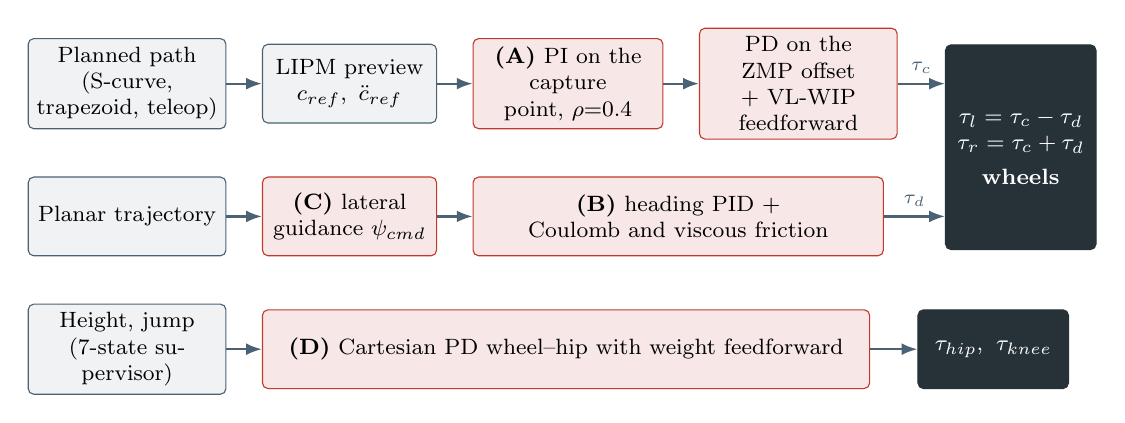
\begin{tikzpicture}[node distance=0.45cm and 0.45cm]
        \node[blk, text width=2.3cm] (path) {Planned path\\(S-curve, trapezoid, teleop)};
        \node[blk, text width=2.0cm, right=of path] (prev) {LIPM preview\\$c_{ref},\ \ddot c_{ref}$};
        \node[pidblk, text width=2.2cm, right=of prev] (cp) {\textbf{(A)} PI on the\\capture point, $\rho{=}0.4$};
        \node[pidblk, text width=2.3cm, right=of cp] (pd) {PD on the ZMP offset\\+ VL-WIP feedforward};
        \node[blk, text width=2.3cm, below=0.6cm of path] (traj) {Planar trajectory};
        \node[pidblk, text width=2.0cm, right=of traj] (lat) {\textbf{(C)} lateral\\guidance $\psi_{cmd}$};
        \node[pidblk, text width=5.0cm, right=of lat] (yaw) {\textbf{(B)} heading PID + Coulomb and viscous friction};
        \node[blk, text width=2.3cm, below=0.6cm of traj] (jump) {Height, jump\\(7-state supervisor)};
        \node[pidblk, text width=7.5cm, right=of jump] (leg) {\textbf{(D)} Cartesian PD wheel--hip with weight feedforward};
        \node[outblk, text width=1.7cm, minimum height=2.6cm, right=0.6cm of pd.east, anchor=north west, yshift=0.5cm] (mix)
            {$\tau_l = \tau_c - \tau_d$\\$\tau_r = \tau_c + \tau_d$\\[3pt]wheels};
        \node[outblk, text width=1.7cm, right=0.6cm of leg] (legout) {$\tau_{hip},\ \tau_{knee}$};
        \draw[arr] (path) -- (prev);
        \draw[arr] (prev) -- (cp);
        \draw[arr] (cp) -- (pd);
        \draw[arr] (pd.east) -- node[above, font=\scriptsize] {$\tau_c$} (pd.east -| mix.west);
        \draw[arr] (traj) -- (lat);
        \draw[arr] (lat) -- (yaw);
        \draw[arr] (yaw.east) -- node[above, font=\scriptsize] {$\tau_d$} (yaw.east -| mix.west);
        \draw[arr] (jump) -- (leg);
        \draw[arr] (leg) -- (legout);
    \end{tikzpicture}
    \caption{Loops of the ZMP-based PID.  State: torso pose from \texttt{/rotino/odom} (ground
    truth) and URDF kinematics, paired by timestamp at 500~Hz; derivatives by finite
    differences.}
    \label{fig:pid_arch}
\end{figure}

\subsection{Loop A: Capture Point $\to$ ZMP $\to$ Torque}

\textbf{Outer loop.}  A PI on the capture-point error, imposing
$\dot\xi = \dot\xi_{ref} - k_\xi e_\xi - k_i\!\int e_\xi$, gives the desired offset between CoM
and ZMP:
\begin{equation}
    s_{des} = s_{ff} - \rho\Big[\frac{\dot e_c}{\omega} + \frac{k_\xi}{\omega}\,e_\xi
              + \frac{k_i}{\omega}\int e_\xi\,\mathrm{d}t\Big],
    \qquad |s_{des}|\le \frac{a_{max}}{\omega^2}.
\end{equation}
\textbf{Inner loop.}  A PD on the offset $s$ moves the contact where it is needed:
\begin{equation}
    \tau_c = \tau_{ff} + K_s\,(s - s_{des}) + K_{sd}\,(\dot s-\dot s_{ff}).
\end{equation}
\textbf{Feedforward.}  From the linearised VL-WIP, the lean and torque that sustain the
reference acceleration in steady state: $s_{ff} = \lambda_s\ddot c_{ref}$,
$\tau_{ff} = \lambda_\tau\ddot c_{ref}$, with $\lambda_s = 21.8$~mm per m/s$^2$.

\begin{table}[H]
    \centering
    \caption{Gains of loop A.}
    \label{tab:pid_gains}
    \begin{tabular}{ll}
        \toprule
        Gain & Value \\
        \midrule
        $K_s$, $K_{sd}$ (per wheel) & 60~Nm/m, 5~Nm\,s/m \\
        $\rho$ (authority) & 0.4 \\
        $k_\xi$, $k_i$ & 1.5~s$^{-1}$, 0.5~s$^{-2}$ \\
        $a_{max}$ & 3~m/s$^2$ (offset $\le$ 59~mm) \\
        $\lambda_s$ & 21.8~mm per m/s$^2$ \\
        Saturation & 10~Nm per wheel \\
        \bottomrule
    \end{tabular}
\end{table}

\subsection{LIPM Preview}

An inverted pendulum cannot follow an acceleration step without leaning first.  The CoM
reference is the \emph{bounded} solution of $\ddot c = \omega^2(c - p_{ref})$, obtained by
filtering the planned contact path with a symmetric kernel that looks about $1/\omega$ into the
future:
\begin{equation}
    c_{ref}(t) = \int_{-\infty}^{+\infty}\frac{\omega}{2}\,e^{-\omega|u|}\,p_{ref}(t+u)\,\mathrm{d}u
    \quad\Rightarrow\quad \ddot c_{ref} = \omega^2\big(c_{ref}-p_{ref}\big).
\end{equation}
The robot leans \emph{before} the acceleration step, as required by the non-minimum phase.  With
dashboard commands the future is unknown, and the current reference acceleration, filtered at
0.1~s, is used instead.  Figure~\ref{fig:lipm} shows the desired and actual ZMP moving behind the
CoM about 0.2~s before the start of a 1~m/s trapezoid.

\begin{figure}[H]
    \centering
    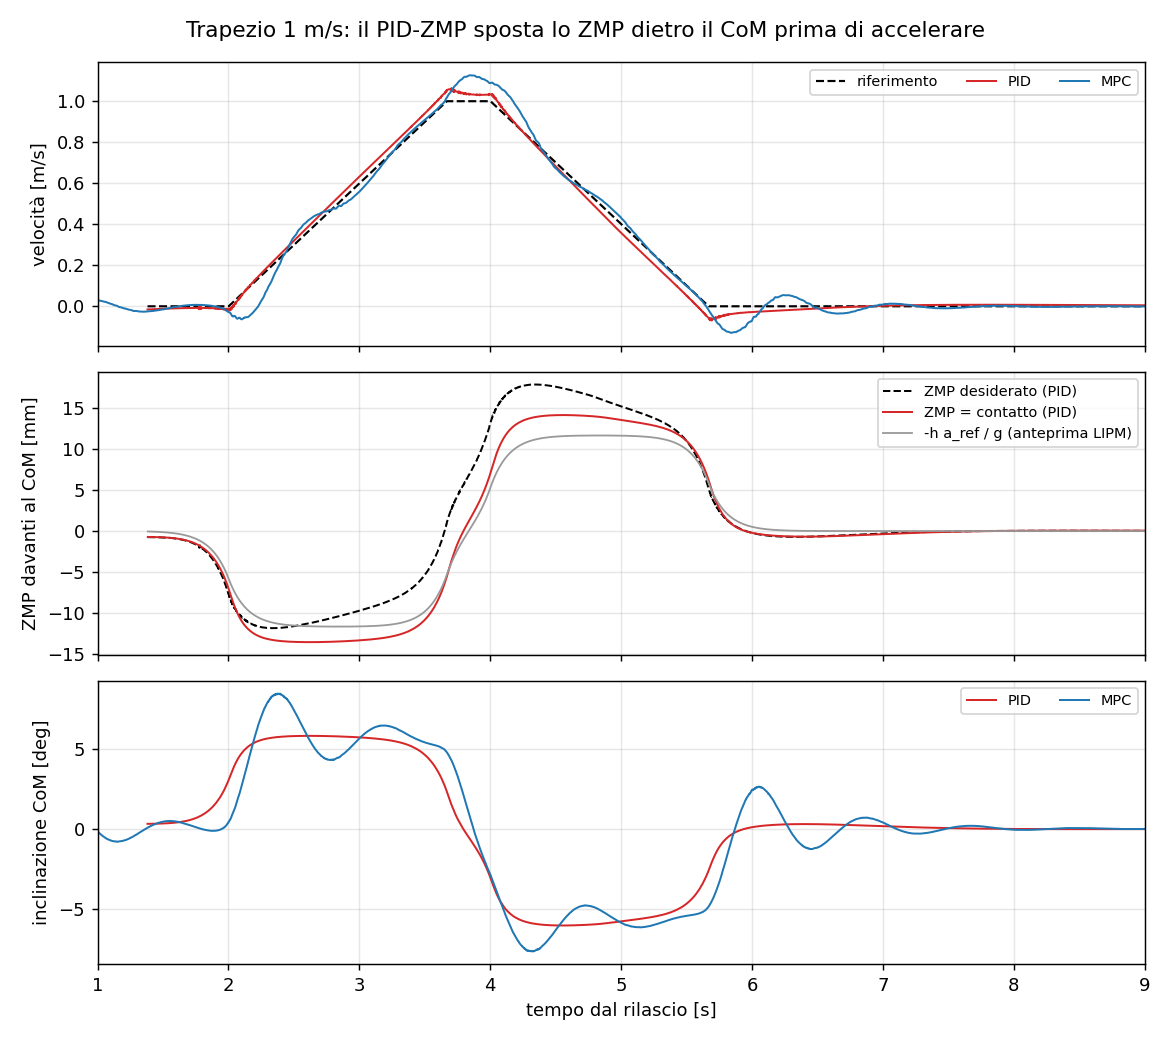
\includegraphics[width=0.78\linewidth]{figures_pid_mpc/pid_zmp_trapezoid.png}
    \caption{Trapezoidal profile at 1~m/s: velocity, desired and actual ZMP of the PID, and CoM
    lean.  The ZMP moves behind the CoM before the wheels accelerate.}
    \label{fig:lipm}
\end{figure}

\subsection{Robust Gain Design}

The gains are not tuned by trial in Gazebo but chosen on the linearised model discretised at
500~Hz.  The pure LIPM cascade assumes an infinitely fast inner loop; with 1--2 samples of
delay and the wheel--pendulum mode at about 10~rad/s, the term $\dot c/\omega$ at full authority
becomes positive feedback on the wheel speed and the cascade is unstable for any sufficiently
high inner gain.  The capture-point correction is therefore passed to the ZMP with
\textbf{authority} $\rho = 0.4$; the residual error is recovered by the integral.

The gains result from robust pole placement over ten cases: mass $\pm20\%$, hip $\pm0.3$~rad
(CoM from crouched to stretched), delay of 1 or 2 samples.  The nominal closed-loop poles are
$-0.5$; $-2.3\pm0.2j$; $-9.8$; $-52$~s$^{-1}$, with \textbf{minimum damping 0.69} over all
cases.  Sixteen offline tests (\texttt{test\_zmp\_balance.py}) verify robust recovery from a
lean, tracking of the trapezoid within 1~cm, rejection of a 2.7~N\,s push, removal of a CoM
offset unknown to the model by the integral, and the LIPM preview.

\subsection{Heading, Lateral Guidance and Legs}

\textbf{Heading (B) and guidance (C).}
\begin{align}
    \tau_d &= K_\psi e_\psi + K_\omega(\dot\psi_{ref}-\dot\psi) + f_c\tanh\!\Big(\frac{\dot\psi_{ref}}{\varepsilon}\Big)
             + f_v\,\dot\psi_{ref} + K_I\!\int e_\psi\,\mathrm{d}t,\\
    \psi_{cmd} &= \psi_{ref} - \arctan(K_{lat}e_\perp)\,\min\!\Big(1,\frac{|v_{ref}|}{0.1}\Big),
\end{align}
with $K_\psi = 1.8$~Nm/rad, $K_\omega = 0.45$~Nm\,s/rad, $K_I = 0.6$, saturation 2.7~Nm and
$K_{lat} = 2$~rad/m.  The Coulomb (0.25~Nm) and viscous (0.10~Nm\,s/rad) scrub friction terms
were identified in Gazebo; they act on the reference, hence without chattering.  Without them
the robot turned in jerks (stick-slip).  The guidance correction fades out near standstill,
because a differential-drive vehicle can only cancel the lateral error while moving.

\textbf{Legs (D).}
\begin{equation}
    \btau_{leg} = J^{T}(\bq)\Big[K_p\,(\bm p_{des}-\bm p) - K_d\,J\bdq + \bm F_{ff}\Big] + b\,\bdq,
    \qquad \bm F_{ff} = -\tfrac12 m_b g\,\hat{\bm z}_b ,
\end{equation}
where $\bm p$ is the wheel centre relative to the hip (\texttt{leg\_fk}).  In stance
$K_p = \operatorname{diag}(1500, 5000)$~N/m and $K_d = \operatorname{diag}(40, 80)$~N\,s/m; in
the jump $(3000, 4000)$; in flight $(800, 800)$ without support.  In joint space this is about
50~Nm/rad: it replaced the joint PD of the MuJoCo port (160--200~Nm/rad), which at 500~Hz
entered a bang-bang limit cycle.

\subsection{Jump Supervisor}

The jump is a seven-state machine (BALANCE $\to$ PRELOAD $\to$ THRUST $\to$ FLIGHT $\to$
LANDING $\to$ RECOVERY $\to$ SETTLE $\to$ BALANCE).  The joint references come from the MuJoCo
controller and are converted into Cartesian wheel positions with \texttt{leg\_fk}.

\begin{table}[H]
    \centering
    \caption{Phases of the jump supervisor.}
    \label{tab:jump}
    \begin{tabular}{lp{6.8cm}p{3.6cm}}
        \toprule
        State & Reference (hip, knee) [rad] & Exit \\
        \midrule
        PRELOAD & $(0,0)\to(+0.12,-0.22)$ in 0.80~s, smoothstep & after 0.80~s \\
        THRUST & $\to(-0.27,+0.44)$ in 0.02~s, $1-(1-\tau)^3$ & take-off, or LANDING after 0.16~s \\
        FLIGHT & pose frozen at take-off, wheels damped & confirmed contact \\
        LANDING & $\to(+0.08,-0.20)$ in 0.80~s, compliant legs & after 0.80~s \\
        RECOVERY / SETTLE & back to $(0,0)$ in 2.0~s, then settling & 0.30~s at rest, or 12~s \\
        \bottomrule
    \end{tabular}
\end{table}

Take-off is confirmed only when four conditions hold together: contact lost (hysteresis,
4~ms), force below threshold, wheel lifted from the ground, and vertical CoM velocity above
0.08~m/s.  During the jump phases the capture-point correction is scaled per phase and the
integral is frozen.

\subsection{Assessment}

\paragraph{Strengths.}  With known references the LIPM preview makes the robot lean in advance
and track without overshoot; the integral on the capture point removes CoM offsets the model
does not know; the law is pure, separated from the ROS node and tested offline on robustness
cases; the gains come from the model (robust poles), not from trial and error in simulation.

\paragraph{Limits and suggestions.}
\begin{itemize}[leftmargin=*]
    \item The state comes from the simulator ground truth, which is not available on a real
          robot and makes the comparison with the MPC asymmetric.
    \item $\rho = 0.4$ is fixed: little authority against pushes.  A $\rho$ scheduled during
          transients would help.
    \item Constraints appear only as saturation ($a_{max}$); the anti-windup does not see the
          reduced limit $10 - |\tau_d|$ in turns.
    \item The telemetry publishes $z_{ref} = z$ on \texttt{/rotino/wbr\_state}, so the height error
          logged by the benchmark is not meaningful for the PID.
    \item The lateral compensation is off: the cylindrical wheel jumps from one edge to the other
          at the inflection of the S-curve; a crowned wheel collision in the URDF would be needed.
\end{itemize}


% ============================================================
\section{MPC + TV-LQR + VMC Controller}
\label{sec:lqr_mpc}

The second controller (\texttt{rotino\_mpc}, files \texttt{controller.py} and \texttt{solvers.py})
implements the architecture of Fig.~4 of~\cite{cui2022}.

\subsection{Why This Architecture}

The paper positions itself between the pure wheeled inverted pendulum (simple, but ignoring the
torso) and whole-body control (complete, but expensive).  It decouples the robot into two simple
models and gives each one the most suitable controller:
\begin{itemize}[leftmargin=*]
    \item \textbf{Balance: fast and unstable.}  A linear model with varying parameters ($l$):
          an LQR recomputed in $l$, which at run time is a matrix--vector product.
    \item \textbf{Posture: slower and constrained.}  Where to put the CoM and how much force to
          ask from the legs, under friction, workspace and $F_z$ limits: an MPC.
    \item \textbf{Legs: virtual model.}  A virtual spring--damper at the foot plus a vertical
          force: no inverse dynamics in stance.
\end{itemize}

\begin{figure}[H]
    \centering
    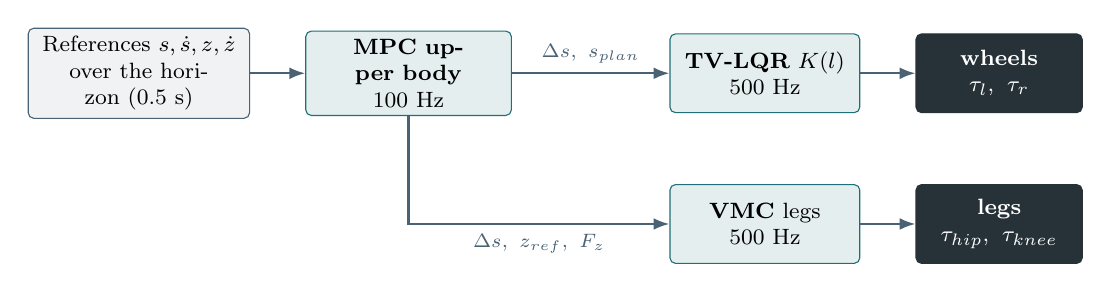
\begin{tikzpicture}[node distance=0.7cm and 0.7cm]
        \node[blk, text width=2.6cm] (ref) {References $s, \dot s, z, \dot z$\\over the horizon (0.5~s)};
        \node[mpcblk, text width=2.4cm, right=of ref] (mpc) {\textbf{MPC upper body}\\100~Hz};
        \node[mpcblk, text width=2.2cm, right=2.0cm of mpc] (lqr) {\textbf{TV-LQR} $K(l)$\\500~Hz};
        \node[outblk, text width=1.9cm, right=of lqr] (wh) {wheels\\$\tau_l,\ \tau_r$};
        \node[mpcblk, text width=2.2cm, below=0.9cm of lqr] (vmc) {\textbf{VMC} legs\\500~Hz};
        \node[outblk, text width=1.9cm, right=of vmc] (lg) {legs\\$\tau_{hip},\ \tau_{knee}$};
        \draw[arr] (ref) -- (mpc);
        \draw[arr] (mpc) -- node[above, font=\scriptsize] {$\Delta s,\ s_{plan}$} (lqr);
        \draw[arr] (lqr) -- (wh);
        \draw[arr] (mpc.south) |- node[pos=0.75, below, font=\scriptsize] {$\Delta s,\ z_{ref},\ F_z$} (vmc.west);
        \draw[arr] (vmc) -- (lg);
    \end{tikzpicture}
    \caption{Architecture of the MPC + TV-LQR + VMC controller.  All three blocks use the state estimated by the Kalman filter from IMU, encoders and leg kinematics.}
    \label{fig:mpc_arch}
\end{figure}

\subsection{TV-LQR Balance Loop}

The cost and the gain are
\begin{gather}
    J = \int_0^\infty\big(\tilde X^{T}Q\tilde X + U^{T}RU\big)\,\mathrm{d}t,\qquad U = -K(l)\,\tilde X,\\
    A^{T}P + PA - PBR^{-1}B^{T}P + Q = 0,\qquad K = R^{-1}B^{T}P,
\end{gather}
with the Riccati equation solved as the stable subspace of the Hamiltonian.  The weights are
\begin{gather}
    Q = \operatorname{diag}(30,\,400,\,80,\,15,\,6,\,2),\\
    R = T^{T}\operatorname{diag}(2,\,100)\,T,\quad T=\begin{bmatrix}\tfrac12&\tfrac12\\-\tfrac12&\tfrac12\end{bmatrix}
    \ \Rightarrow\ U^{T}RU = 2\tau_c^2+100\,\tau_d^2 .
\end{gather}

\begin{table}[H]
    \centering
    \caption{Bryson reading of $Q$: $1/\sqrt{q_{ii}}$ is the deviation that costs one unit.}
    \label{tab:bryson}
    \begin{tabular}{lcccccc}
        \toprule
        State & $s$ & $\theta$ & $\varphi$ & $\dot s$ & $\dot\theta$ & $\dot\varphi$ \\
        \midrule
        $q_{ii}$ & 30 & 400 & 80 & 15 & 6 & 2 \\
        $1/\sqrt{q_{ii}}$ & 0.18~m & 0.050~rad ($2.9\dgr$) & 0.11~rad & 0.26~m/s & 0.41~rad/s & 0.71~rad/s \\
        \bottomrule
    \end{tabular}
\end{table}

The lean has priority and the position is accepted within tens of centimetres: the robot
yields in translation so as not to fall.  The weight on the common mode coincides with $R = I$;
with this $R$ the Riccati problem splits into a sagittal and a yaw part.  The differential mode
costs 50 times more because of a torsional resonance of the stance legs at about 76~rad/s
(torso yaw inertia on the VMC springs): with $R_d = 100$ the yaw loop crosses over at
15.4~rad/s, a fifth of the resonance.

\subsection{Gains, Poles and Scheduling on $l$}

In the nominal pose
\begin{equation}
    K(l_0)=\begin{bmatrix}-3.87&-20.28&-0.89&-5.64&-2.78&-0.21\\-3.87&-20.28&+0.89&-5.64&-2.78&+0.21\end{bmatrix}.
\end{equation}
$K_s = 3.873 = \sqrt{30/2} = \sqrt{q_s/r_c}$ does not depend on $l$; likewise the yaw gain
$0.894 = \sqrt{q_\varphi/r_d}$.  \texttt{LQRSchedule} computes $K$ on 25 poses (each with its own
$I_y$) and interpolates linearly in $l$; the sagittal poles hardly move
(Table~\ref{tab:lqr_sched}), which is the purpose of the schedule.  The fast pole at $-180$~rad/s
lies beyond the bandwidth of the $\dot\theta$ filter, so in the real loop it is set by the filter
and the sampling.  The slow pair $-1.08\pm0.68j$ ($\zeta = 0.85$) is the return to position seen
after a push.  The interpolation at frozen $l$ is justified as long as $l$ varies slowly, which
is not the case during the jump thrust, where $\dot l$ is ignored.

\begin{table}[H]
    \centering
    \caption{TV-LQR gains and sagittal poles along the pose grid.}
    \label{tab:lqr_sched}
    \begin{tabular}{ccccl}
        \toprule
        $l$ [m] & $K_\theta$ [Nm/rad] & $K_{\dot\theta}$ & $K_{\dot s}$ & Sagittal poles \\
        \midrule
        0.219 & 21.22 & 3.13 & 5.51 & $-139.9$; $-8.06$; $-1.15\pm0.68j$ \\
        \textbf{0.163} & \textbf{20.28} & \textbf{2.78} & \textbf{5.64} & $\bm{-179.5}$; $\bm{-8.13}$; $\bm{-1.08\pm0.68j}$ \\
        0.074 & 18.43 & 2.33 & 6.32 & $-281.1$; $-8.16$; $-0.86\pm0.63j$ \\
        \bottomrule
    \end{tabular}
\end{table}

\subsection{Upper-Body MPC}

The MPC predicts the CoM with two independent double integrators, obtained by freezing the
coefficient $(g+\ddot z)/h$ over the horizon (eq.~9 of~\cite{cui2022}):
\begin{align}
    \begin{bmatrix}s\\ \dot s\end{bmatrix}_{k+1} &= \begin{bmatrix}1&\Delta T\\0&1\end{bmatrix}\begin{bmatrix}s\\ \dot s\end{bmatrix}_k
    + \begin{bmatrix}\Delta T^2/2\\ \Delta T\end{bmatrix}\frac{g+\ddot z_{ref}}{h}\,\Delta s_k,\\
    \begin{bmatrix}z\\ \dot z\end{bmatrix}_{k+1} &= \begin{bmatrix}1&\Delta T\\0&1\end{bmatrix}\begin{bmatrix}z\\ \dot z\end{bmatrix}_k
    + \begin{bmatrix}\Delta T^2/2\\ \Delta T\end{bmatrix}\Big(\frac{F_{z,k}}{m_b}-g\Big).
\end{align}
With $\Delta T = 0.02$~s and $N = 25$ (0.5~s horizon, updated at 100~Hz), the condensed QP
\begin{equation}
    \min_{U}\ \tfrac12 U^{T}HU + g^{T}U\quad \text{s.t.}\ \ \bm{l}\le U\le \bm{h},\qquad
    H = \Gamma^{T}\bar S\,\Gamma + W I,\quad g = \Gamma^{T}\bar S\,(\Phi x_0 + C - x_{ref})
\end{equation}
(see~\cite{rawlings2017}) has only box constraints, so a projected accelerated gradient is enough: FISTA~\cite{beck2009},
60 iterations, step $1/\lambda_{max}(H)$, warm-started from the previous solution shifted by one
node.  Compared with the paper, the discretisation is exact (ZOH) instead of Euler, and the QPs
are two and decoupled.

\textbf{Weights.}  Horizontal: $S_h = \operatorname{diag}(50, 20)$ on $(s,\dot s)$, $W_h = 200$ on
$\Delta s$, so that 1~cm of $\Delta s$ costs as much as 2~cm of position error.  Vertical:
$S_v = \operatorname{diag}(5000, 150)$, $W_v = 2\cdot10^{-3}$: a stiff height, because the VMC has
no vertical spring in stance.

\subsection{Constraints and Reference for the LQR}

\begin{gather}
    |\Delta s| \le \min\!\Big(\mu z,\ \sqrt{L_{max}^2-z_b^2},\ 0.03\Big),\qquad
    0.3\,m_b g \le F_z \le \{3;\,6\}\,m_b g,\\
    \theta_{ref}=\operatorname{atan2}(\Delta s, z_{ref}).
\end{gather}
In the nominal pose $\mu z = 0.357$~m and $\sqrt{L_{max}^2 - z_b^2} = 0.184$~m: \textbf{the active
constraint is always the 3~cm cap}, added in the implementation, which limits $\theta_{ref}$ to
$10.48\dgr$ and the steady deceleration to $g_{st}\cdot 0.03/0.162 = 1.13$~m/s$^2$.  The friction
limit of the paper would allow $\arctan(2.2) = 65\dgr$ of lean.  $F_{min} = 0.3\,m_bg$ keeps the
contact in the plan; the upper bound rises from 3 to 6 times the weight during the jump thrust.

The LQR does not track the raw reference but the MPC plan:
\begin{equation}
    X_{ref}=\big[\,s_{plan}-\Delta s,\ \operatorname{atan2}(\Delta s,z_{ref}),\ \varphi_{ref},\ \dot s_{plan},\ 0,\ \dot\varphi_{ref}\,\big]^{T}.
\end{equation}
$\Delta s$ (filtered at 19~ms) is used twice: as $\theta_{ref}$ and axle set-back for the LQR, and
as the foot position relative to the CoM for the VMC.  Wheels and legs thus realise the same
displacement.

\subsection{VMC, State Estimation and Yaw}

\textbf{VMC.}  For each leg
\begin{equation}
    \btau_{leg} = J^{T}\big[K_p(\bm p_d-\bm p_f) + K_d(\bm v_d-\bm v_f) + \bm F_{ff}\big] + b_{leg}\,\bdq,\qquad
    \bm F_{ff}=-\tfrac12F_z\,\hat{\bm z}_b,
\end{equation}
with $K_p = \operatorname{diag}(1500, 0)$~N/m and $K_d = \operatorname{diag}(40, 15)$~N\,s/m in
stance.  $K_{p,z} = 0$: the height is regulated by the MPC through $F_z$, and a spring in parallel
would be a second regulator on the same quantity.  Horizontally the foot converges in 27~ms, much
faster than the CoM.

\textbf{Kalman filter.}  Three scalar filters (one per world axis), state $[p, v]$, driven by the
IMU acceleration and corrected by wheel odometry plus leg kinematics:
\begin{gather}
    x_{k|k-1} = F x_{k-1} + \Gamma a_{w,k},\qquad P_{k|k-1} = FP_{k-1}F^{T}+Q,\\
    K_k = P_{k|k-1}\big(P_{k|k-1}+R\big)^{-1},\qquad x_{k} = x_{k|k-1}+K_k\big(y_k-x_{k|k-1}\big),
\end{gather}
with $q_a = 0.5$~(m/s$^2$)$^2$ and $R = \operatorname{diag}(10^{-4}, 10^{-3})$.  The fusion time
constants are 45~ms (IMU) and 280~ms (odometry); the correction runs only in stance.

\textbf{Yaw.}  The $\varphi$ row of the TV-LQR plus Coulomb and viscous friction feedforward and
an integral with a 0.035~rad dead zone; the differential torque is limited to 2.5~Nm and the
common mode to $10 - |\tau_d|$.

\subsection{Assessment}

\paragraph{Strengths.}  Anticipation of the references (0.5~s horizon in a non-minimum-phase
system); constraints enforced in the plan rather than saturated afterwards; a single synthesis
for $F_z$ covering stance, height changes and jump thrust; a realistic estimate (IMU + Kalman)
that transfers to a real robot.

\paragraph{Limits and suggestions.}
\begin{itemize}[leftmargin=*]
    \item No integral action in the sagittal plane: on the reduced model, a constant 3~N push
          leaves a 0.65~m steady-state error.
    \item The prediction model has no pitch: the MPC does not know that moving the CoM first
          requires tilting the pendulum, and leaves it entirely to the LQR.
    \item The 3~cm cap makes the friction constraint of the paper inactive and limits the
          deceleration.
    \item Suggestions: an integral state or a disturbance model in the QP; a lean constraint
          depending on $h$; prediction on the full VL-WIP.
\end{itemize}


% ============================================================
\section{Comparison Framework}
\label{sec:comparison}

\subsection{Methodology}

The comparison changes only the controller node.  \texttt{robot.launch.py} starts the
simulation, the robot and the scenario, and receives from the control package only the name of
its executable: same URDF, same Gazebo world, same torque actuation at 500~Hz, same scenario
arguments.  The campaign is regenerated with \texttt{ros2 run rotino\_benchmark suite}.  One
difference of conditions must be kept in mind: the PID reads the ground-truth state, the MPC an
estimated one.

\subsection{Architectures Side by Side}

\begin{table}[H]
    \centering
    \caption{Synthesis of the two architectures.}
    \label{tab:synth}
    \begin{tabular}{p{3.0cm}p{5.4cm}p{5.4cm}}
        \toprule
        & PID with ZMP & MPC + TV-LQR + VMC \\
        \midrule
        Balance state & ground truth, unfiltered derivatives & IMU + Kalman + kinematics \\
        Wheel law & PI on capture point $\to$ ZMP $\to$ PD & LQR scheduled on $l$ \\
        Use of the model & VL-WIP feedforward, LIPM preview & LQR (VL-WIP) + MPC (lumped mass) \\
        Translation & LIPM preview + capture-point integral & MPC with preview + LQR on the plan \\
        Lean limit & ZMP offset $\le a_{max}/\omega^2$ (3~m/s$^2$) & $\Delta s \le 3$~cm $\to 10.48\dgr$ \\
        Yaw & PID + friction & LQR ($R_d = 100$) + friction + integral \\
        Legs & Cartesian PD, 1500/5000~N/m & VMC, $K_{p,z} = 0$, support from $F_z$ \\
        Integral action & capture point, yaw & yaw only \\
        Sagittal poles & $-0.5$; $-2.3\pm0.2j$; $-9.8$; $-52$ & $-8.13$; $-1.08\pm0.68j$ \\
        \bottomrule
    \end{tabular}
\end{table}

\subsection{Benchmark Scenarios and Figures}

The comparison is organised in four families of scenarios (Table~\ref{tab:scenarios}).  For
each family the figures below indicate the plot to be inserted from
\texttt{benchmark\_runs/suite\_pid\_mpc/} and the metrics to discuss.  In the benchmark plots the
PID is drawn in red and the MPC in blue.

\begin{table}[H]
    \centering
    \caption{Benchmark scenarios.}
    \label{tab:scenarios}
    \begin{tabular}{lp{10.5cm}}
        \toprule
        Family & Scenarios \\
        \midrule
        Disturbances & push of 2.7~N\,s backwards on the torso 4~s after release; vertical jump at 4~s, then balance \\
        Tracking & trapezoid: 2~m at 1~m/s with 0.6~m/s$^2$; back and forth: 1~m in 8~s \\
        S-curves & 3~m S with 0.6~m lateral offset in 12~s, and fast version: 1~m in 5~s \\
        Balance and height & balance at rest after release; sinusoidal height $\pm3$~cm with 2.2~s period \\
        \bottomrule
    \end{tabular}
\end{table}

\newcommand{\plotslot}[2]{%
    \tikz\node[todo]{\textbf{Figure to be inserted}\\[4pt]\texttt{\detokenize{#1}}\\[6pt]Metrics: #2};}

\begin{figure}[H]
    \centering
    \plotslot{spinta/plots/disturbo_e_fase.png}{peak pitch, recovery time, maximum position error}\hfill
    \plotslot{salto/plots/assetto.png}{CoM rise, peak pitch, recovery time}
    \caption{Disturbances: push on the torso and jump.  \emph{Key message: to be written after
    inserting the plots.}}
    \label{fig:cmp_dist}
\end{figure}

\begin{figure}[H]
    \centering
    \plotslot{trapezio/plots/inseguimento.png}{rms position and velocity error, peak pitch}\hfill
    \plotslot{va_e_vieni/plots/inseguimento.png}{rms position error, rms wheel torque}
    \caption{Tracking: trapezoid and back and forth.  \emph{Key message: to be written.}}
    \label{fig:cmp_track}
\end{figure}

\begin{figure}[H]
    \centering
    \plotslot{curva_S_veloce/plots/zmp_lateral.png}{maximum lateral ZMP / (d/2), minimum wheel load}\hfill
    \plotslot{curva_S/plots/inseguimento.png}{rms position error, peak pitch}
    \caption{S-curves: tracking and lateral ZMP.  \emph{Key message: to be written.}}
    \label{fig:cmp_s}
\end{figure}

\begin{figure}[H]
    \centering
    \plotslot{equilibrio/plots/coppie_ruote.png}{steady rms pitch, rms wheel torque}\hfill
    \plotslot{altezza/plots/assetto.png}{rms height oscillation, rms pitch}\\[8pt]
    \plotslot{riepilogo.png}{balance over the 31 key metrics}
    \caption{Balance, height change and overall balance of the metrics.  \emph{Key message: to be
    written.}}
    \label{fig:cmp_bal}
\end{figure}


% ============================================================
\section{Contributions with Respect to Class Topics}
\label{sec:contributions}

\begin{itemize}[leftmargin=*]
    \item \textbf{Configuration space and DOFs:} DOF count of the floating-base robot, topology
          $SE(3)\times\Real^4\times T^2$, holonomic and Pfaffian constraints, Brockett's theorem.
    \item \textbf{Dynamic modelling:} symbolic Euler--Lagrange model with the parameters of the
          URDF, Christoffel-symbol construction of $\bC$, automatic checks of symmetry, positive
          definiteness and passivity, input matrix verified with a rigid-motion test.
    \item \textbf{Underactuated control:} non-collocated partial feedback linearisation,
          reduction to the VL-WIP, analysis of instability and non-minimum phase.
    \item \textbf{ZMP-based balance:} cart-table model, capture point, LIPM preview, robust pole
          placement on the discretised model with delay.
    \item \textbf{Optimal control (LQR/MPC):} TV-LQR scheduled on leg length, condensed QP with
          FISTA at 100~Hz, common/differential torque decomposition.
    \item \textbf{Leg control and estimation:} Cartesian PD and virtual model control through the
          Jacobian transpose; linear Kalman filter fusing IMU, odometry and leg kinematics.
\end{itemize}


% ============================================================
\section{Conclusions}
\label{sec:conclusions}

This report presented the modelling and control of RoTino with the parameters of its URDF, from
the configuration space to two complete control laws.

\begin{enumerate}
    \item The four-coordinate Lagrangian model, recomputed symbolically with the real parameters,
          reproduces the CoM of the library used by the controllers and satisfies the structural
          properties of a mechanical system.  The analysis also exposed two inconsistencies in
          the MATLAB scripts (signs of $\bB$ in \texttt{wbr\_terms.m}, missing $-\partial T/\partial\bq$
          in \texttt{init.m}).
    \item The reduced VL-WIP shows the two structural difficulties: an unstable pole at
          10.3~rad/s and real zeros at $\pm6.2$~rad/s.  Both controllers use the lean as the input
          of the translation.
    \item The PID, redesigned around the ZMP, moves the contact with the wheels under a
          capture-point loop of reduced authority; the LIPM preview lets it lean before
          accelerating.  Its gains come from robust pole placement on the discretised model.
    \item The MPC + TV-LQR + VMC handles constraints and future references explicitly, with a
          realistic state estimate, but has no sagittal integral action and a prediction model
          without pitch.
    \item The quantitative comparison is set up in Section~\ref{sec:comparison} and will be
          completed with the plots of the benchmark suite.
\end{enumerate}

Future work: a crowned wheel collision to enable the lateral ZMP compensation, a scheduled
authority $\rho$ and IMU-based estimation for the PID, an integral state and a pitch-aware
prediction model for the MPC, and validation on hardware.


% ============================================================
\begin{thebibliography}{9}

\bibitem{cui2022}
Z.\ Cui, Y.\ Xin, S.\ Liu, X.\ Rong, and Y.\ Li,
``Modeling and Control of a Wheeled Biped Robot,''
\emph{Micromachines}, vol.\ 13, no.\ 5, p.\ 747, 2022.

\bibitem{kajita2003}
S.\ Kajita, F.\ Kanehiro, K.\ Kaneko, K.\ Fujiwara, K.\ Harada, K.\ Yokoi, and H.\ Hirukawa,
``Biped walking pattern generation by using preview control of zero-moment point,''
in \emph{Proc.\ IEEE ICRA}, 2003, pp.\ 1620--1626.

\bibitem{englsberger2011}
J.\ Englsberger, C.\ Ott, M.\ A.\ Roa, A.\ Albu-Sch\"affer, and G.\ Hirzinger,
``Bipedal walking control based on Capture Point dynamics,''
in \emph{Proc.\ IEEE/RSJ IROS}, 2011, pp.\ 4420--4427.

\bibitem{brockett1983}
R.\ W.\ Brockett,
``Asymptotic stability and feedback stabilization,''
in \emph{Differential Geometric Control Theory}, Birkh\"auser, 1983, pp.\ 181--191.

\bibitem{beck2009}
A.\ Beck and M.\ Teboulle,
``A fast iterative shrinkage-thresholding algorithm for linear inverse problems,''
\emph{SIAM J.\ Imaging Sciences}, vol.\ 2, no.\ 1, pp.\ 183--202, 2009.

\bibitem{rawlings2017}
J.\ B.\ Rawlings, D.\ Q.\ Mayne, and M.\ Diehl,
\emph{Model Predictive Control: Theory, Computation, and Design}, 2nd~ed.,
Nob~Hill~Publishing, 2017.

\bibitem{siciliano2009}
B.\ Siciliano, L.\ Sciavicco, L.\ Villani, and G.\ Oriolo,
\emph{Robotics: Modelling, Planning and Control},
Springer, 2009.

\end{thebibliography}

\end{document}
